\documentclass[tikz,border=4pt]{standalone}
\usepackage{amsmath}
\definecolor{curveblue}{HTML}{245C86}
\begin{document}
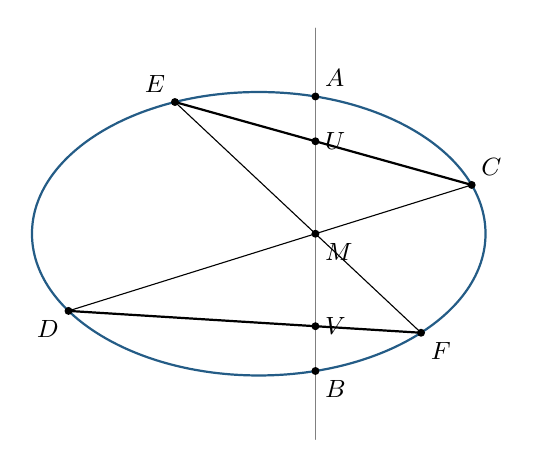
\begin{tikzpicture}[font=\small,line cap=round,scale=1.8]
\draw[curveblue,thick](-.4,0)ellipse[x radius=1.6,y radius=1];
\coordinate(C)at(1.102111,0.344410);
\coordinate(D)at(-1.742111,-0.544410);
\coordinate(E)at(-0.991184,0.929235);
\coordinate(F)at(0.745030,-0.698466);
\coordinate(A)at(0.000000,0.968246);
\coordinate(B)at(0.000000,-0.968246);
\coordinate(U)at(0.000000,0.652318);
\coordinate(V)at(0.000000,-0.652318);
\coordinate(M)at(0.000000,0.000000);
\draw[gray](0,-1.45)--(0,1.45);
\draw(C)--(D) (E)--(F);
\draw[thick](C)--(U)--(E) (D)--(V)--(F);
\foreach \name/\pos in {A/above right,B/below right,C/above right,D/below left,E/above left,F/below right,U/right,V/right,M/below right}{\fill(\name)circle(.8pt)node[\pos]{$\name$};}
\end{tikzpicture}
\end{document}
